% ****** Start of file aipsamp.tex ******
%
%   This file is part of the AIP files in the AIP distribution for REVTeX 4.
%   Version 4.1 of REVTeX, October 2009
%
%   Copyright (c) 2009 American Institute of Physics.
%
%   See the AIP README file for restrictions and more information.
%
% TeX'ing this file requires that you have AMS-LaTeX 2.0 installed
% as well as the rest of the prerequisites for REVTeX 4.1
% 
% It also requires running BibTeX. The commands are as follows:
%
%  1)  latex  aipsamp
%  2)  bibtex aipsamp
%  3)  latex  aipsamp
%  4)  latex  aipsamp
%
% Use this file as a source of example code for your aip document.
% Use the file aiptemplate.tex as a template for your document.
\documentclass[%
 aip,
 % onecolumn,
% jmp,
% bmf,
% sd,
 % rsi,
 amsmath,amssymb,
%preprint,%
 reprint,%
%author-year,%
%author-numerical,%
% Conference Proceedings
floatfix,
% tikz,
]{revtex4-1}

\usepackage{graphicx}% Include figure files
\usepackage[utf8]{inputenc}
\usepackage[T1]{fontenc}
\usepackage{mathptmx}
\usepackage{tikz}
\usetikzlibrary{arrows,decorations.markings,decorations.pathmorphing, patterns,shapes}
\usepackage{dcolumn}% Align table columns on decimal point
\usepackage{bm}% bold math
\usepackage{float}
%\usepackage[mathlines]{lineno}% Enable numbering of text and display math
%\linenumbers\relax % Commence numbering lines

\begin{document}
\preprint{AIP/123-QED}

\title[]{The Busch Helical Method: \\ Measuring the Ratio of an Electron's Charge to Mass}
% Force line breaks with \\

\author{Jared Baur and Ben Sappey}
 % \altaffiliation[Also at ]{Physics Department, XYZ University.}%Lines break automatically or can be forced with \\
% \author{Ben Sappey}%
% \affiliation{ 
% Authors' institution and/or address%\\This line break forced with \textbackslash\textbackslash
% }%

\date{\today}% It is always \today, today,
             %  but any date may be explicitly specified


\begin{abstract}

	The charge to mass ratio for an electron is widely accepted to be $1.758 \times 10^{11}$ C/kg. In this experiment, the Busch-Helical method is used to determine this ratio. This method uses a solenoid and cathode ray tube in order to send an electron beam down a helical path. The electrons are illuminated on a phosphor screen at the end of the cathode ray tube, and can be focused down to a small point by adjusting the parameters of the current through the solenoid. Using the adjusted parameters of the solenoid and accelerating voltage used to initialize the electron beam, the charge to mass ratio can be calculated. This experiment resulted in a charge to mass ratio of $(1.82 \pm 0.07) \times 10^{11}$ C/kg, which is consistent with the accepted value. A separate regression analysis resulted in a charge to mass ratio of $(1.84 \pm 0.06) \times 10^{11}$ C/kg, which is not consistent with the accepted value. This is likely due to the nature of regression analysis and best-fit lines, which compromise the consistency of the data with the accepted value for finding the best-fit between the data itself.

\end{abstract}

\maketitle


\onecolumngrid

\section{\label{sec:level1}Objective}

	Measure the charge-to-mass ratio of the electron using the Busch Helical Method.

\section{\label{sec:level2}Introduction}

In 1922, Busch developed a method of measuring the ratio of an electron's charge to its mass. This method involved focusing a divergent beam of electrons via a magnetic field. The electrons travel through a cathode ray tube in a specific trajectory. The trajectory of an electron in the presence of a magnetic field, when the electron is not moving parallel to the field, is in a helical motion. For mathematical purposes, this helical motion can be described as traveling along the surface of a cylinder. The electrons start from a hot cathode at the base of the tube. They pass through an anode with a velocity that depends on the potential difference between the cathode and the anode. This potential difference is called the "accelerating voltage". The applied magnetic field in the solenoid cause the beam of electrons to travel in the previously mentioned helical motion, completing a certain number of loops until hitting the fluorescent screen on the end of the cathode ray tube. The result from this process is a light that is emitted from the screen that changes with size as the magnetic field is changed. The original Busch design for this experiment had auxiliary magnets strategically placed around the cathode ray tube (instead of a solenoid) in order to produce the desired magnetic field\cite{Stranathan1942}.

In order to obtain the ratio of an electron's charge to its mass, let us consider a single electron moving with velocity $v$ as it exits the anode with an angle $\beta$ to the axis of the cathode ray tube. The magnetic field will influence the electron's trajectory, however only in the motion that is perpendicular to the magentic field. Thus, the longitudinal component of the velocity, $v \cos{\beta}$ will remain constant and the perpendicular component, $v \sin{\beta}$ will vary. The electron will go through a helical motion around the axis of the tube, all while traveling down the tube at a constant velocity. It will then pass through the center axis as it completes one helical revolution. The electron's perpendicular velocity component can be expressed as

\begin{figure}[H]
		\centering
		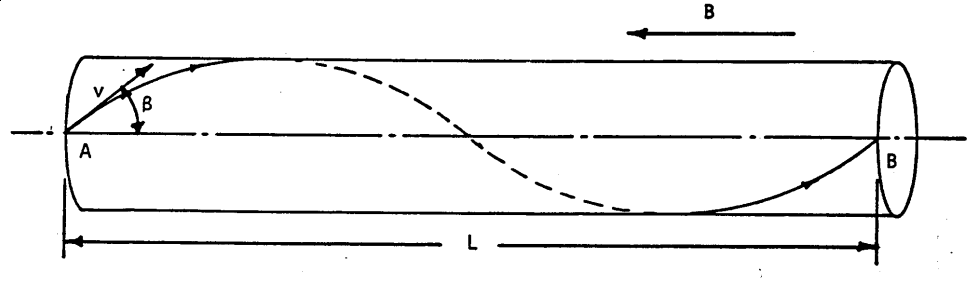
\includegraphics[scale=0.5]{electrontrajectory.png}
		\caption{Path of electrons in the solenoid. Electrons leave the cathode ray anode with a velocity $v$ at an angle $\beta$.}
	\end{figure}

\begin{equation}
	v \sin{\beta} = \frac{m(v \sin{\beta})^2}{eHR}
\end{equation}
 
\noindent where $H$ is the magnetic field, $m$ is the mass of the electron, $e$ is the charge of the electron, and $R$ is the radius of the helical path taken by the electron. The time $t$ for the electron to complete one revolution of this helix is expressed in Equation 2.

\begin{equation}
	t = \frac{2 \pi m}{H e}
\end{equation}

\noindent Solving for $R$ in either of these equations and plugging into the other will give a simplified form for the time $t$ of one revolution.

\begin{equation}
	t = \frac{2 \pi m}{H e}
\end{equation}

\noindent Since Equation 3 is independent of the perpendicular velocity, all electrons, regardless of longitudinal velocity, will complete one revolution in the same amount of time. If all electrons sent through the cathode have the same velocity (influenced by the accelerating voltage), then they will hit the fluorescent screen at the same time, thus creating a focused image on the screen. The time for the electrons to travel from the anode to the screen is expressed in Equation 4. In this equation, $L$ is the distance from the anode to the fluorescent screen.

\begin{equation}
	t = \frac{L}{v \cos{\beta}}
\end{equation}

\noindent When the magnetic field is adjusted so that there is a focused point on the screen, the time for the electron to reach the screen and the time for it to complete one revolution are equal. Thus, Equation 3 and 4 can be set equal to one another. Solving for the ratio $e/m$ gives equation 5. 

\begin{equation}
	\frac{e}{m} = \frac{2 \pi V \cos{\beta}}{\mu_0 H L}
\end{equation}

\noindent The velocity of the electron can be found by analyzing the kinetic energy $V e = 1/2 m v^2$, where $V$ is the accelerating voltage. By solving for $v$ and replacing into Equation 5, we get Equation 6. The angle $\beta$ is significantly small, so the term $\cos^2{\beta}$ is considered unity. The constant $\mu_0$ is the permeability of free space, a measure of the amount of resistance encountered when forming a magnetic field in a classical vacuum. The accepted value for $\mu_0$ is $4 \pi \times 10^{-7}$ H/m.

\begin{equation}
	\frac{e}{m} = \frac{8 \pi^2 V}{\mu_0^2 H^2 L^2} \cos^2{\beta}
\end{equation}


\section{\label{sec:level3}Apparatus and Methods}

The apparatus consists of a cathode ray tube and a solenoid. The cathode ray anode emits electrons with the assistance of a high voltage power supply (Kepco Model Power Supply). The cathode ray tube is placed in the center of the solenoid with the axes of the tube and solenoid aligned. An accelerating voltage is applied to the cathode ray tube that accelerates electrons in a beam. A voltage applied to the intensity control grid by a separate power supply (Heathkit Regulated Power Supply Model PS-4) reduces the current of the emitted electron beam. The solenoid's magnetic field provides a curved, helical path for the electron beam to follow in the cathode tube. The solenoid's current is reversible via a homemade switch; when reversed, the magnetic field is reversed and the helical orientation of the electron beam is flipped (clockwise or counterclockwise).

	\begin{figure}[H]
		\centering
		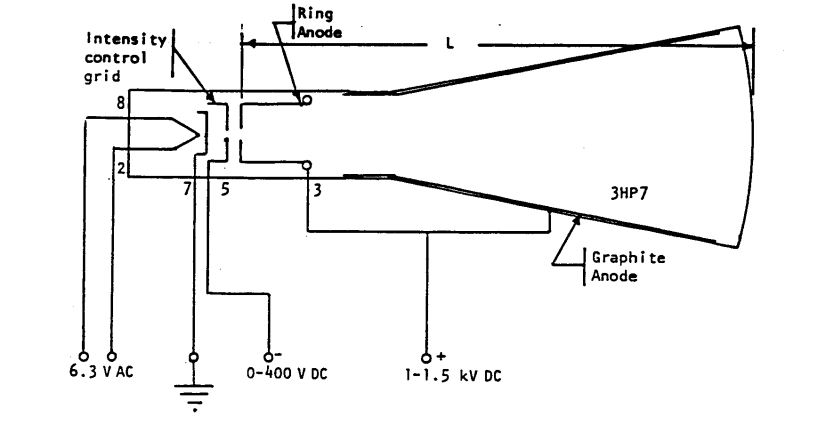
\includegraphics[scale=0.5]{cathoderaytube.png}
		\caption{Cathode ray tube schematic. Electrons are emitted from the anode and travel a distance $L$ through the cathode tube.}
	\end{figure}
Before beginning the experiment, measurements of the apparatus were made in order to obtain the values needed for calculations. The cathode ray's length $L$ was measured (used in Equation 7) with the use of a cathetometer. The cathetometer was chosen to make this measurement since it can easily be used to measure distances of objects where the measuring tool cannot be placed close to the point of interest. The cathetometer was used to measure the distance from the anode to the end of the tube (length $L$ shown in Figure 2). This length is defined as the distance from the anode to the phosphor screen that is the point at which the electrons are illuminated in the cathode tube. The phosphor screen is actually embedded underneath a glass of measurable thickness, which also required the use of a cathetometer to measure. In order to measure the glass thickness, the pinpoint of a thumbtack was placed on the surface of the glass. The microscope on the cathetometer was focused on this pinpoint and the reading on the cathetometer scale was taken. Next, the focus of the microscope was adjusted to the phosphor screen under the glass. Once the phosphor was in focus, the cathetometer scale reading was noted. The difference between these two readings represent the thickness of the glass, which was then used to calculate the actual length $L$ of the cathode ray tube (from the anode to the phosphor screen).

The magnetic field in a solenoid is given by Equation 7, where $H$ is the magnitude of the magnetic field, $n$ is the density of turns for the length of the solenoid (number of turns per unit length), $I$ is the current, and $\beta$ is the angle subtended at the center of the solenoid by the outer edge of the solenoid and its axis\cite{oxymanual}. The turn density was measured by counting the number of turns for a select unit of length, then extrapolating this small turn density to the total length of the solenoid. The angle $\beta$ was found by measuring the angle from the end of the solenoid (on the axis through its center) to the middle of the solenoid (on the solenoid's edge). The orientation of the solenoid was determined based on the earth's magnetic field. If the solenoid is placed perpendicularly to earth's magnetic field, then there would be no interference from earth's magnetic field on the electron beam. This effect is seen in the Lorentz force: $\bold{F} = q\bold{v} \times \bold{B}$; since the tangential velocity vector of the electron beam is parallel to earth's magnetic field when the solenoid is perpendicular to it, there is no outside interference. A magnetic compass was used to place the solenoid in its correct orientation.

\begin{equation}
	H = nI\cos{\theta}
\end{equation}

Before applying an accelerating voltage to the cathode ray tube, the intensity control power supply was turned on to about 300 volts. This prevented any future damage to the phosphor screen. Subsequent damage would reduce the phosphor's ability to illuminate the electron beam upon contact with the screen. Next, the accelerating voltage was applied to the cathode ray tube by turning on the main power supply to about 600 volts. A multimeter (Fluke Model 77 IV) was used to measure this voltage. Steps of about 75 volts were taken to vary the accelerating voltage throughout this experiment. The main power supply outputs its readings as kilovolts, so a volt box (Leeds \& Northup Co. Model 7593) was used to create a multiplier to convert kilovolts to centivolts (multiplier of 10,000). This allowed for a more accurate reading from the multimeter since larger values were output to the multimeter, thus allowing for the tens and ones place to be measured more accurately (since they are now visible on the multimeter screen). A current $I$ was sent down the solenoid with another power supply (Lambda Regulated Power Supply Model LR 344A FM), which was varied based on the focus of the elecron beam on the phosphor screen. For low voltage values, scanning the magnetic field through its entire range given by the current $I$, the elecron beam makes many turns in the cathode ray tube. This is seen experimentally by the focus of the beam on the phosphor screen increasing and decreasing as it travels in a circular path. The number of turns of the electron beam was reduced to one for each trial by finding the lowest possible current for which the electron beam was at focus on the phosphor screen.

For each step in the accelerating voltage, the optimal focus point of the electron beam was found, and the corresponding current from the solenoid's power supply was recorded. This current was measured with the help of a Biddle-Gray standard resistor that provides a resistance to the voltage provided from the power supply. By having this fixed resistance, the current is measured using Ohm's Law $I=V/R$. A switch is used to change the input to the multimeter from the accelerating voltage power supply to the solenoid power supply in order to measure this voltage. Ten trials were ran and data was obtained for the accelerating voltage and the magnetic field in the solenoid, for which the ratio of $e/m$ was calculated.

\section{\label{sec:level4}Data Analysis}

A voltage of 300 volts was applied to the intensity control grid to prevent damage to the phosphor screen in the cathode ray tube. Then, a voltage varying from 603 to 1520 volts was applied as an accelerating voltage to the tube. The uncertainty in this voltage, measured by the multimeter, is 0.3\% + 1 digit (given by the Fluke multimeter manual\cite{Fluke}). With the solenoid power supply on, the phosphor screen was observed with a spot on it. This spot was focused by adjusting the solenoid's current to the lowest possible value while still remaining focused. The voltage through intensity control grid was adjusted for when the spot became significantly intense. The voltage through the solenoid was also measured with the multimeter by flipping the input switch to the multimeter from the accelerating voltage power supply to the solenoid power supply. The uncertainty for the voltage through the solenoid is also 0.3\% + 1 digit. The standard resistor has a constant resistance of 0.1 ohms with an uncertainty of 0.04\%. The data for the accelerating voltage, solenoid voltage, solenoid current, and subsequent magnetic field (Equation 7) is presented in Table 1.

The uncertainty for all calculations in this experiment is obtained using Taylor's Error Analysis\cite{Taylor1996}. The uncertainty for the current $I$ through the solenoid was obtained using Equation 7, where $\delta x$ is the uncertainty in value $x$. The uncertainty for the magnetic field follows the same form, given in Equation 8. In Equation 8, the uncertainties for $n$ and $\theta$ are listed. These are instrumental uncertainties that follow from the implement used in measuring them. For the turn density $n$, a meter stick was used to measure the total length of the solenoid, which was used to extrapolate the number of turns for the entire length of the solenoid. The uncertainty used from the meter stick was 1 mm. The turn density was measured to be $1220 \pm 20$ turns/meter. The length of the solenoid was measured to be $0.602 \pm 0.01$ m. A meter stick was also used to calculate $\theta$, since the angle subtended at the center of the solenoid is $\theta = \tan^{-1}\big({\frac{2 \times \text{solenoid diameter}}{\text{solenoid length}}}\big)$. The angle $\theta$ was measured to be $0.17 \pm 0.02$ radians with a solenoid diameter of $0.105 \pm 0.01$ m. The meter stick was used to measure the solenoid diameter as well as the length from calculating the turn density (uncertainty of 1 mm). The uncertainty of the charge to mass ratio calculated is simply the sum of $\delta H$ and $\delta I$, shown in Equation 10. In Table 1, the uncertainty for the charge to mass ratio is only listed once because the calculated uncertainty is the same for each trial.


\begin{equation}
	\frac{\delta I}{\lvert I \rvert} \approx \frac{\delta V}{\lvert V \rvert} + \frac{\delta R}{\lvert R \rvert}
\end{equation}

\begin{equation}
	\frac{\delta H}{\lvert H \rvert} \approx \frac{\delta n}{\lvert n \rvert} + \frac{\delta I}{\lvert I \rvert} + \frac{\delta \theta}{\lvert \theta \rvert}
\end{equation}

\begin{table}
	\centering
	\caption{Accelerating voltage and solenoid current used to calculate the magnetic field in the solenoid. The charge to mass ratio is shown, as calculated from Equation 6. The uncertainty for the charge to mass ratio is the same throughout all trials.}
	\begin{ruledtabular}
	\begin{tabular}{lllll}
		Accelerating&Solenoid&Solenoid&Magnetic&Charge to Mass\\
		Voltage ($V$)&Voltage ($V$)&Current ($A$)&Field ($Oe$)&Ratio ($\times 10^{11}$)\\
	\hline
	    603   $\pm$ 2     & 0.1920 $\pm$ 0.0006 & 1.920 $\pm$ 0.007 & 2308  $\pm$ 81 & 1.75 $\pm$ 0.07\\
	    674   $\pm$ 2     & 0.2016 $\pm$ 0.0006 & 2.016 $\pm$ 0.007 & 2423  $\pm$ 85 & 1.78\\
	    753   $\pm$ 2     & 0.2078 $\pm$ 0.0006 & 2.078 $\pm$ 0.007 & 2497  $\pm$ 88 & 1.87\\
	    828   $\pm$ 2     & 0.2236 $\pm$ 0.0007 & 2.236 $\pm$ 0.008 & 2687  $\pm$ 94 & 1.78\\
	    908   $\pm$ 3     & 0.2312 $\pm$ 0.0007 & 2.312 $\pm$ 0.008 & 2779  $\pm$ 97 & 1.82\\
	    980   $\pm$ 3     & 0.2428 $\pm$ 0.0007 & 2.428 $\pm$ 0.008 & 2918  $\pm$ 102 & 1.78\\
	    1060  $\pm$ 3     & 0.2489 $\pm$ 0.0007 & 2.489 $\pm$ 0.008 & 2991  $\pm$ 105 & 1.83\\
	    1142  $\pm$ 3     & 0.2583 $\pm$ 0.0008 & 2.583 $\pm$ 0.009 & 3104  $\pm$ 109 & 1.83\\
	    1213  $\pm$ 4     & 0.2629 $\pm$ 0.0008 & 2.629 $\pm$ 0.009 & 3160  $\pm$ 111 & 1.88\\
	    1294  $\pm$ 4     & 0.2745 $\pm$ 0.0008 & 2.745 $\pm$ 0.009 & 3299  $\pm$ 116 & 1.84\\
	    1364  $\pm$ 4     & 0.2824 $\pm$ 0.0008 & 2.824 $\pm$ 0.010 & 3394  $\pm$ 119 & 1.83\\
	    1447  $\pm$ 4     & 0.2987 $\pm$ 0.0009 & 2.987 $\pm$ 0.010 & 3590  $\pm$ 126 & 1.74\\
	    1520  $\pm$ 5     & 0.2945 $\pm$ 0.0009 & 2.945 $\pm$ 0.010 & 3539  $\pm$ 124 & 1.88\\
	    \hline
	    Average &	&	&	& 1.82 $\pm$ 0.07\\
	\end{tabular}%
	\end{ruledtabular}
\end{table}%

\begin{equation}
	\frac{\delta e/m}{\lvert e/m \rvert} \approx \frac{\delta n}{\lvert n \rvert} + \frac{\delta I}{\lvert I \rvert} + \frac{\delta \theta}{\lvert \theta \rvert} + \frac{\delta V}{\lvert V \rvert} + \frac{\delta R}{\lvert R \rvert}
\end{equation}


Figure 3 depicts the relationship between the accelerating voltage $V$ and the squared solenoid current $I^2$, the exact relationship from Equation 6. Since the rest of the variables in Equation 6 are constant, the charge to mass ratio can be determined from this point. A regression analysis on the data in Figure 3 presents a best fit line of slope $172.23 \pm 5.21$. The value of the rest of the contents of Equation 6, $8\pi^2/\mu_0^2n^2\cos^2{\theta}L^2$, is equal to 0.0107. When combined with the slope of the regression, we get $1.84 \pm 0.06$.

\begin{figure}[H]
	\centering
	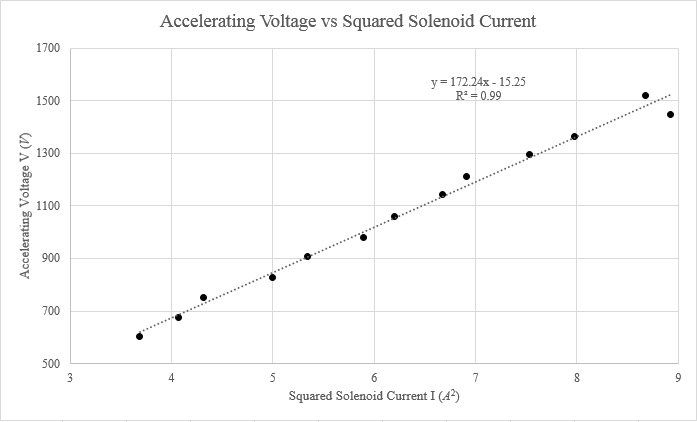
\includegraphics[scale=0.9]{graph.png}
	\caption{Relationship between $V$ and $I^2$. The y-intercept was not set to zero so that the best-fit line would not be compromised.}
\end{figure}

\section{\label{sec:level5}Conclusion}

The charge to mass ratio found from the regression on the data presented in Table 1 is $(1.84 \pm 0.06) \times 10^{11}$ C/kg. The same ratio found by averaging the results from calculating with Equation 6 is $(1.82 \pm 0.07) \times 10^{11}$ C/kg. These two experimentally obtained ratios are consistent with each other, and the latter ratio is consistent with the accepted value of e/m, $1.758 \times 10^{11}$ C/kg. The regression-driven result is likely inconsistent with the accepted value because of the y-intercept that is output from the best-fit line. Since the y-intercept is negative, increasing it to zero would decrease the slope, thus decreasing the ratio and (likely) making it consistent with the accepted value of charge to mass ratio. This was not done, however, since altering the y-intercept would compromise the best-fit line and the high coefficient of determination ($R^2=0.99$). 

The Busch-Helical method is a relatively old method that, as shown, still produces accurate values for the charge to mass ratio of an electron as compared to the accepted values of today. The accuracy of this experiment in particular could have been improved in accuracy with a more precise method of aligning the solenoid perpendicularly to earth's magnetic field to prevent any interference with the electron beam. Another source of inaccuracy in this experiment was the turn density of the solenoid. Since there were such a large number of turns, measuring the turns for a small amount of length and extrapolating for a significantly larger distance is not the most precise method of measurement. Nonetheless, a consistent value for the charge to mass ratio of an electron was obtained.

\nocite{*}
\bibliography{main}% Produces the bibliography via BibTeX.
\end{document}
